%---------------------------------------------------------------------
%
%    Project Name: Radar System Signal Process Software Design Discuss
%
%---------------------------------------------------------------------
%
%               created by LuoMin <luomin5417@gmail.com>
%
%                       Last-modified: 2018-12-14
%
%---------------------------------------------------------------------

\documentclass[a4paper,12pt]{report}
\usepackage{etex}
\usepackage{ctex}
%\usepackage{xeCJK}
\usepackage{times}
\usepackage{setspace}
\usepackage{fancyhdr}
\usepackage{graphicx}
\usepackage{wrapfig}
\usepackage{array}  
\usepackage{fontspec,xunicode,xltxtra}
\usepackage{titlesec}
\usepackage{titletoc}
\usepackage[titletoc]{appendix}
\usepackage[top=30mm,bottom=30mm,left=20mm,right=20mm]{geometry}
\usepackage{cite}
\usepackage{listings}
\usepackage{caption,subcaption}
\usepackage[framed,numbered,autolinebreaks,useliterate]{mcode} % 插入代码
\usepackage{xeboiboites}
\usepackage{amsmath,amssymb}
\usepackage{hyperref}
\usepackage{float}

\usepackage{xcolor}
\usepackage{tcolorbox}

\usepackage{enumerate}
\usepackage[font=small,labelsep=space]{caption}
\usepackage{multirow}

\RequirePackage{tkz-network}

\hypersetup{hidelinks}

\XeTeXlinebreaklocale "zh"
\XeTeXlinebreakskip = 0pt plus 1pt minus 0.1pt

%---------------------------------------------------------------------
%	页眉页脚设置
%---------------------------------------------------------------------
\fancypagestyle{plain}{
    \pagestyle{fancy}      %改变章节首页页眉
}

\pagestyle{fancy}
\lhead{\kaishu~宜通华盛~}
\rhead{\kaishu~研发部~}
\cfoot{\thepage}

%---------------------------------------------------------------------
%	章节标题设置
%---------------------------------------------------------------------
\titleformat{\chapter}{\centering\zihao{-1}\heiti}{第\chinese{chapter}章}{1em}{}
\titlespacing{\chapter}{0pt}{*0}{*6}

%---------------------------------------------------------------------
%	摘要标题设置
%---------------------------------------------------------------------
\renewcommand{\abstractname}{\zihao{-3} 摘\quad 要}

%---------------------------------------------------------------------
%	参考文献设置
%---------------------------------------------------------------------
\renewcommand{\bibname}{\zihao{2}{\hspace{\fill}参\hspace{0.5em}考\hspace{0.5em}文\hspace{0.5em}献\hspace{\fill}}}

%---------------------------------------------------------------------
%	引用文献设置为上标
%---------------------------------------------------------------------
\makeatletter
\def\@cite#1#2{\textsuperscript{[{#1\if@tempswa , #2\fi}]}}
\makeatother

%---------------------------------------------------------------------
%	目录页设置
%---------------------------------------------------------------------
\titlecontents{chapter}[0em]{\songti\zihao{-4}}{\thecontentslabel\ }{}
{\hspace{.5em}\titlerule*[4pt]{$\cdot$}\contentspage}
\titlecontents{section}[2em]{\vspace{0.1\baselineskip}\songti\zihao{-4}}{\thecontentslabel\ }{}
{\hspace{.5em}\titlerule*[4pt]{$\cdot$}\contentspage}
\titlecontents{subsection}[4em]{\vspace{0.1\baselineskip}\songti\zihao{-4}}{\thecontentslabel\ }{}
{\hspace{.5em}\titlerule*[4pt]{$\cdot$}\contentspage}

%---------------------------------------------------------------------
%	公式设置
%---------------------------------------------------------------------
%%define the newthem environment
\newboxedtheorem[small box style={fill=blue!20,draw=black, 
    rounded corners},
    big box style={fill=blue!10,draw=orange,thick,rounded corners},
    headfont=\bfseries]%
    {proposition}{公式}{somecounter} 

%---------------------------------------------------------------------
%   生成大纲
%---------------------------------------------------------------------

\begin{document}
%---------------------------------------------------------------------
%	封面设置
%---------------------------------------------------------------------
\begin{titlepage}
    \begin{center}
        
    
\includegraphics[width=0.8\textwidth]{figure//etws.png}\\
    \vspace{40mm}
    \textbf{\zihao{2}\kaishu{ETWS-1810雷达信处}}\\[0.8cm]
    \textbf{\zihao{2}\kaishu{软件设计讨论}}\\[3cm]
    
    \vspace{\fill}
    
\setlength{\extrarowheight}{3mm}
{\songti\zihao{3}	
\begin{tabular}{rl}
    
    {\makebox[5\ccwd][s]{部\qquad 门:}}& ~\kaishu 研发部\\
    
    {\makebox[5\ccwd][s]{编\qquad 制:}}& ~\kaishu 罗敏 \\ 

    {\makebox[5\ccwd][s]{版\qquad 本:}}& ~\kaishu 1.0 \\

\end{tabular}
 }\\[2cm]
\vspace{\fill}
\zihao{4}
使用\LaTeX 撰写于\today
    \end{center}	
\end{titlepage}

%---------------------------------------------------------------------
%  摘要页
%---------------------------------------------------------------------
\begin{abstract}
\begin{spacing}{1.5}
    {\zihao{-4}
    本文主要是关于雷达系统自研信号处理分系统软件设计讨论,目的是确定信号处理分系统软件和
    算法处理部分的详细工作。因对于信号处理部分均是从零起步,一个好的实现方案和计划更显的
    尤为重要,本文从信号处理分系统输出目标出发,逐步详细阐述各个设计目标的计算和实现过程。

    \textbf{关键字}:\quad 雷达系统 \quad 信号处理 \quad 算法 \quad 实现
    }
\end{spacing}
\end{abstract}

%---------------------------------------------------------------------
%  目录页
%---------------------------------------------------------------------
\tableofcontents % 生成目录

%---------------------------------------------------------------------
%  第一章
%---------------------------------------------------------------------
\chapter{设计目标}
\setcounter{page}{1}
\begin{spacing}{1.5}
\songti\zihao{-4}

\section{输出指标}
本节主要是对雷达信号处理分系统的设计指标进行确认,确定设计输出的指标之后,才能够更好的针
对设计指标进行软件设计和规划。
\begin{figure}[hbtp]
    \centering
    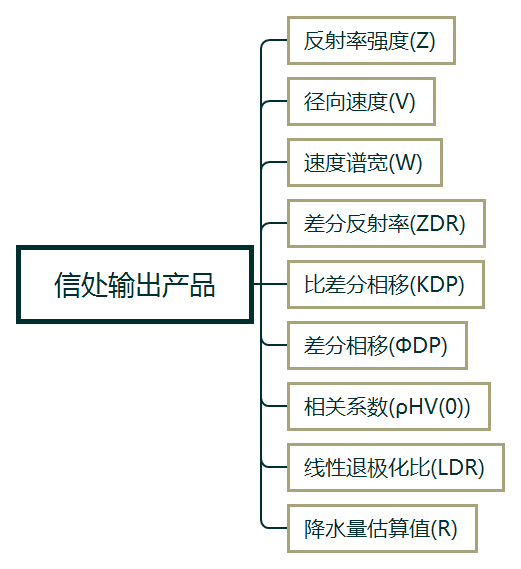
\includegraphics [width=0.5\textwidth]{figure//output.png}
    \caption{信处输出原始产品}\label{output}
\end{figure}
在图1.1中根据《X波段双偏振天气雷达改造升级项目立项报告》列了一下信处分系统应该要输出的原
始产品。


\section{硬件架构}
目前硬件架构已经基本确认,具体如图1.2所示主要采用AD板+接口板+X86板的方案。AD板与接口板
之间采用SIRO接口连接,接口板与X86板之间采用PCIe3.0接口连接。如图所示,AD板主要负责下变
频、抽取、滤波等工作,接口板则负责接收AD板采集的数据,然后对数据进行DBF、脉冲压缩等处理,
同时需要控制伺服、波控等组件,X86板则接收接口板处理后的数据做后半段的信号数据处理,最终输
出上一节中提到的输出指标。
\begin{figure}[hbtp]
    \centering
    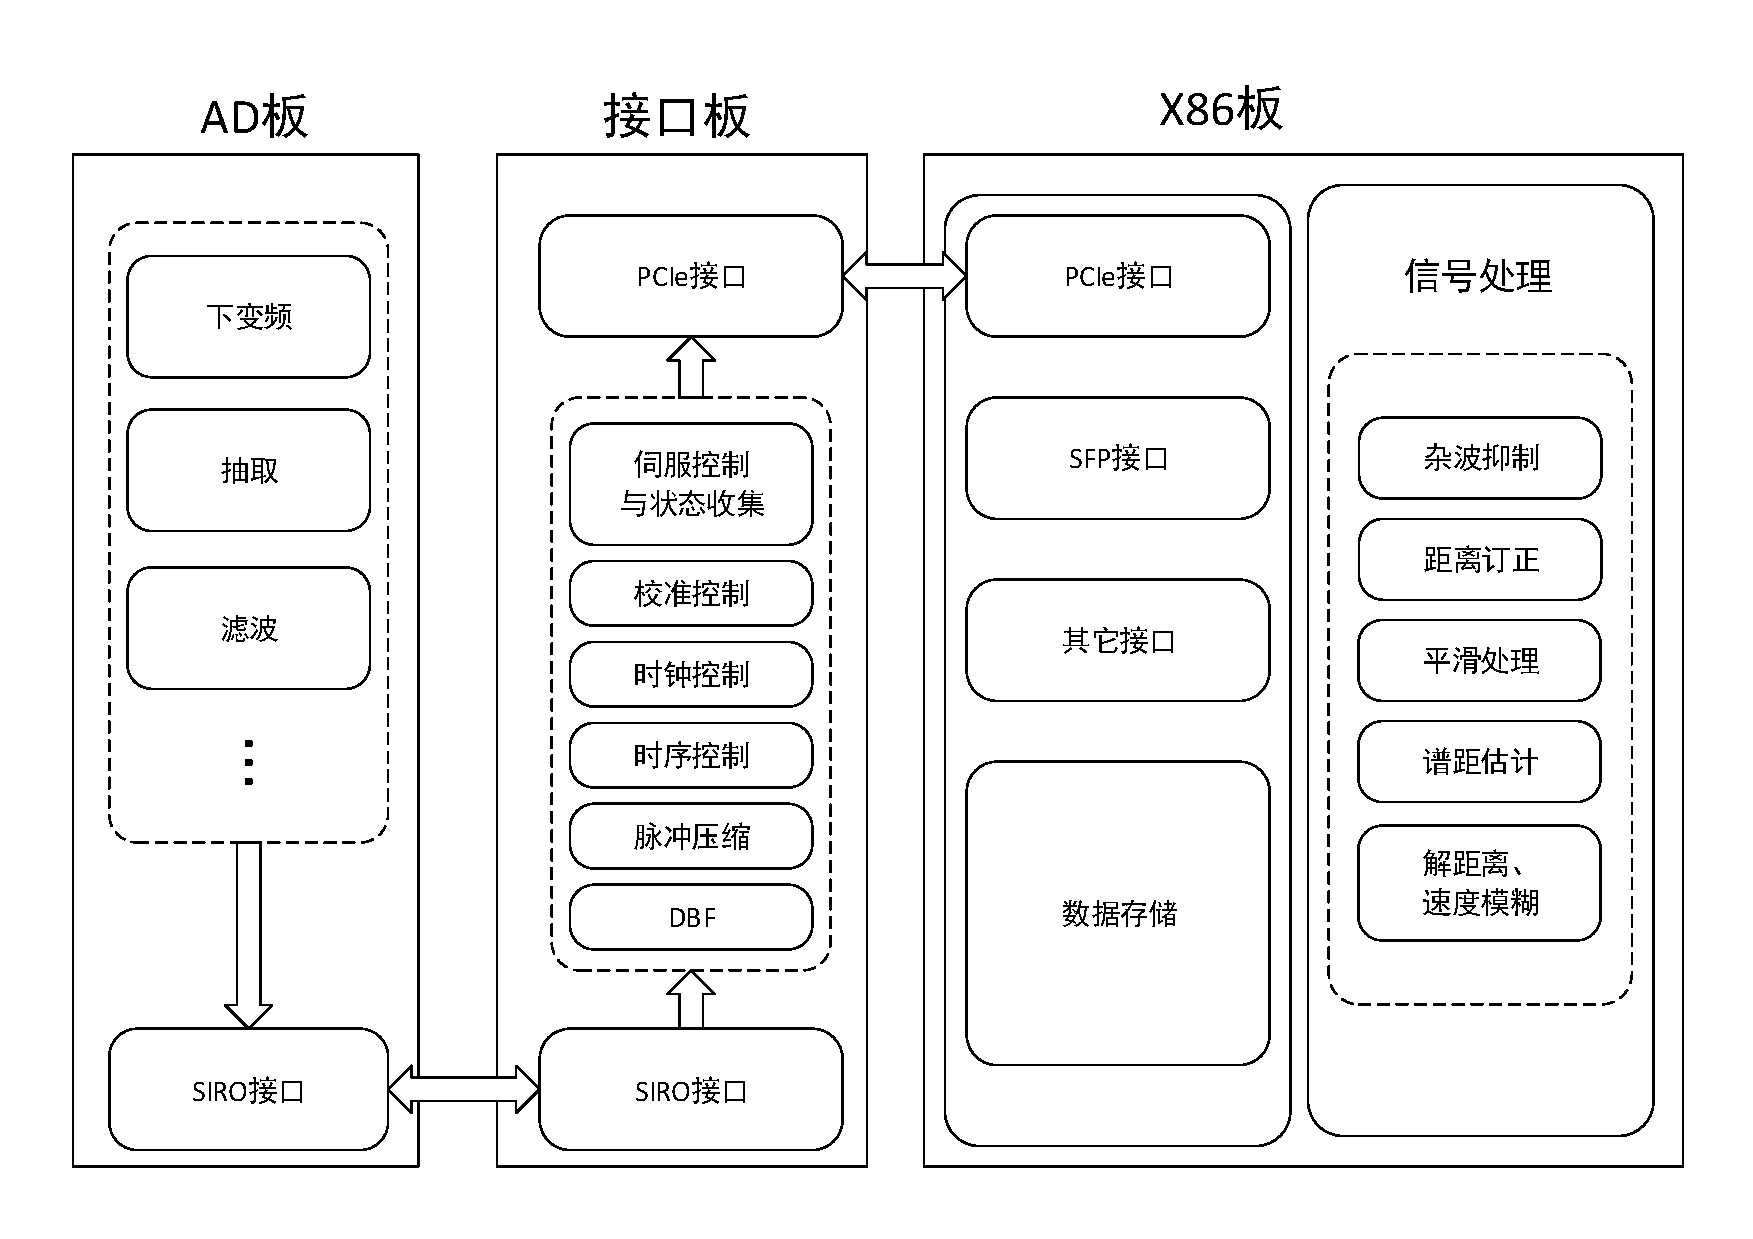
\includegraphics [width=0.8\textwidth]{figure//HardDesign.pdf}
    \caption{硬件设计}\label{HardDesign}
\end{figure}

因本文主要讨论软件的设计实现,主要会聚焦于X86板的信号处理部分,目前接口板与X86板的数据通
道已经是对接过,可以从接口板读取相关数据,后续的工作便是两个主要的工作:
\begin{itemize}
    \itemsep=3pt
    \parskip=0pt
    \setlength{\itemindent}{1em}
    \item 设计接口板与X86板接收数据的协议
    \item 处理理接收到的数据
\end{itemize}


%\begin{table}[hbtp]
%	\centering
%	\caption{软件功能要求}
%	\begin{tabular}{lp{3cm}p{4cm}p{4cm}}
%	\hline
%	模块    & 软件            & 功能                 &         备注\\
%	\hline
%    \multirow{2}{*}{网关}     & 系统软件& 网关的基本通信功能& 基于Openwrt开源系统\\
%    %\cline{2-4}
%	~  & 远程控制软件    & 设备远程配置       & 基于curl工具进行开发\\
%    %\hline
%
%    服务器  & 服务器软件  & 采集数据建立通信通道 & 定制开发\\
%    %\hline          
%
%	管理软件    & 设备管理软件 & 管理网关和设备     & 使用浏览器远程登录服务器 \\
%	\hline          
%	\end{tabular}
%	\label{tab:Cost_evalua}
%\end{table}

\end{spacing}

%---------------------------------------------------------------------
%  第二章
%---------------------------------------------------------------------
\chapter{设计原理}
\begin{spacing}{1.5}
\songti\zihao{-4}

\section{数据模型}
\subsection{三维数据模型}
需要对雷达回波进行数据处理,首先要将回波数据抽象成一个数据处理模型,在这里采用了三维数据
块作为一个数据处理模型\cite{FundamentalsOfRadarSignalProcessing},这一处理方法引用自
雷达信号处理基础第三章,基本处理模型如图2.1所示:
\begin{figure}[hbtp]
    \centering
    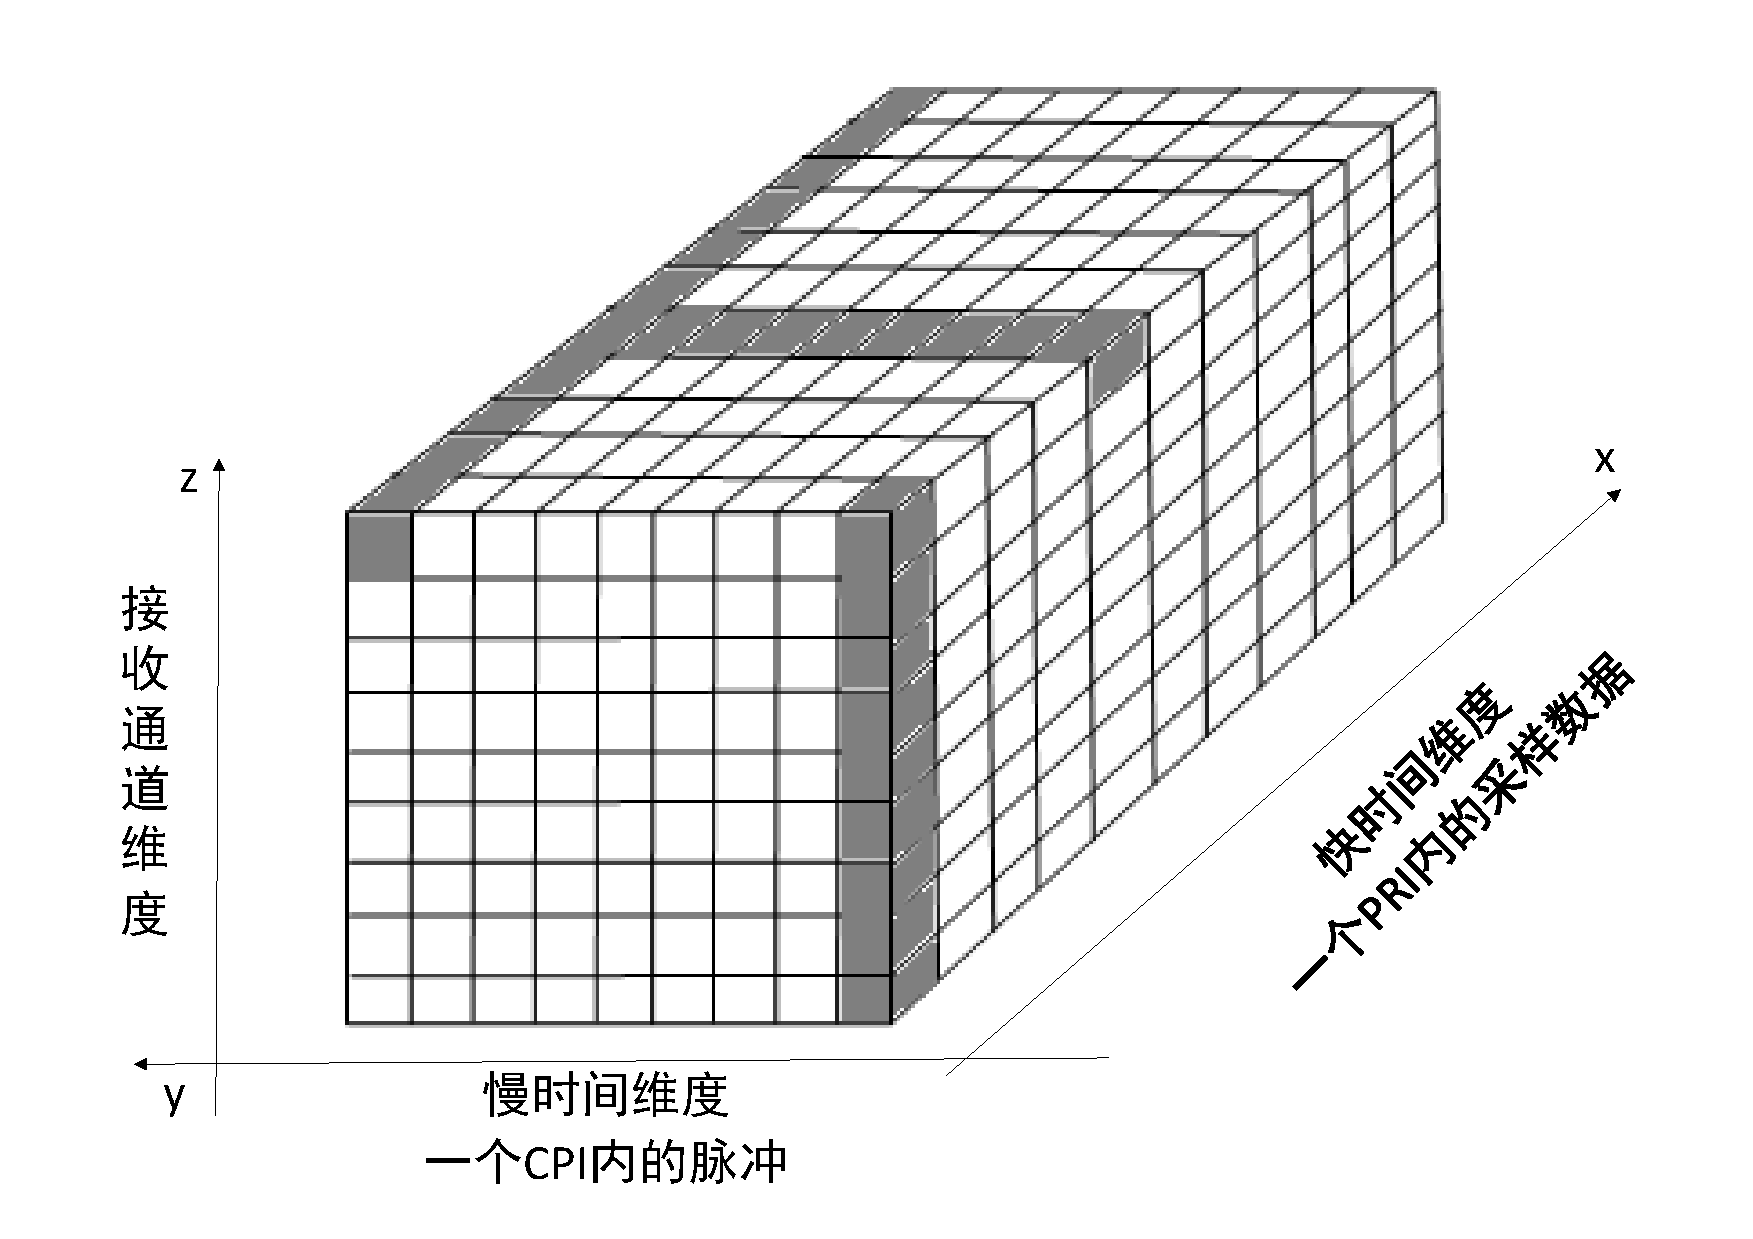
\includegraphics [width=1.0\textwidth]{figure//DataBlock.pdf}
    \caption{信号处理数据块}\label{DataBlock}
\end{figure}

可以看到,在上图中的x轴方向标注为快时间维度,本质就是一个PRI(脉冲重复间隔)内的回波
采样数据.y轴标注为慢时间维度,本质是一个CPI(相干处理间隔)内的多组回波数据。z轴标注的是
接收通道维度,本质就是对应天线的接收通道数目。

\subsection{数据模型理解}
上一节是介绍了基本的数据模型,在本节中还需要深入的理解一下设计的数据模型,在图2.2中,针
对数据模型的三个维度进行了进一步的标注。
\begin{figure}[hbtp]
    \centering
    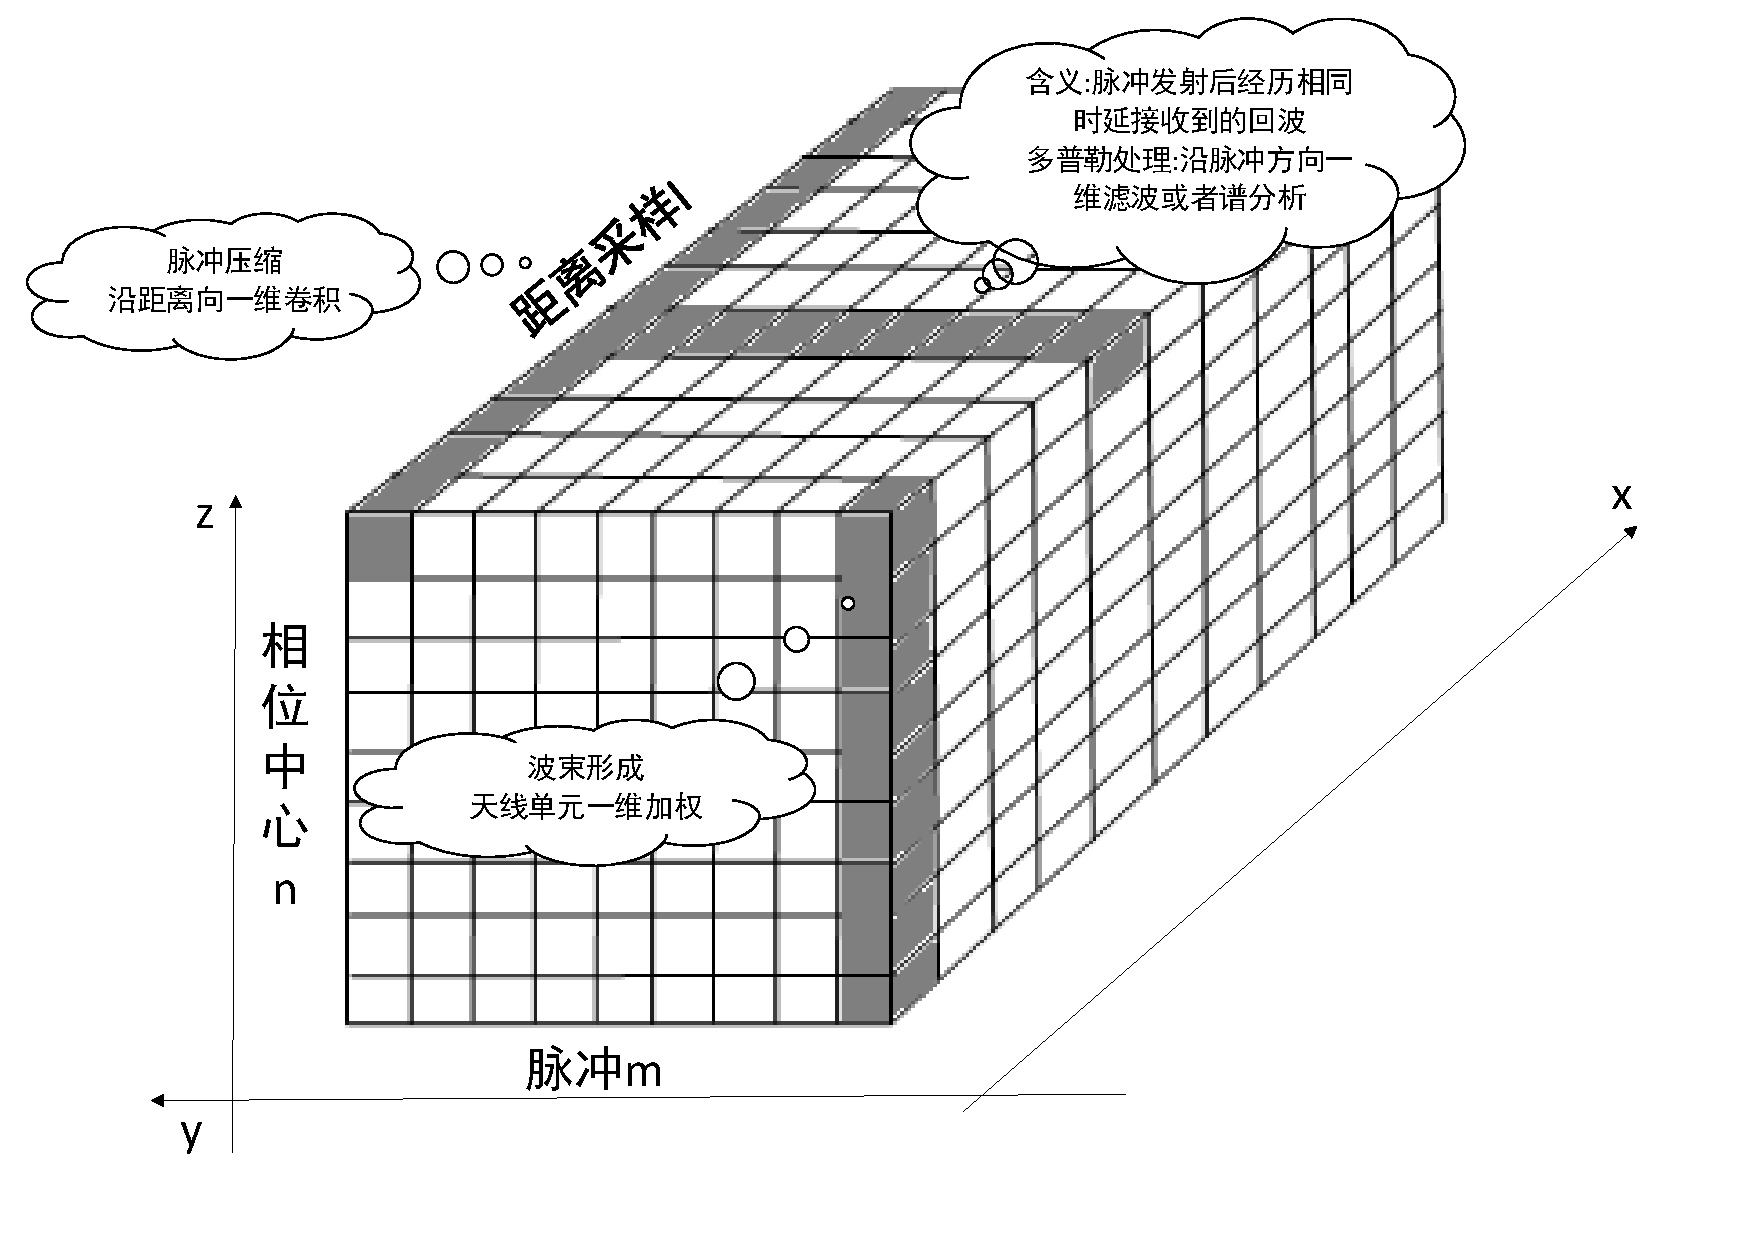
\includegraphics [width=1.0\textwidth]{figure//DataBlock2.pdf}
    \caption{信号处理数据块}\label{DataBlock2}
\end{figure}

x轴方向标注为距离采样l,脉冲压缩处理便是在这一维度做处理,而多普勒处理则是沿y轴方向,y轴
方向还有一个很重要的含义,便是脉冲发射后经历相同时延接收到的回波,z轴代表不同的接收通道,
不同的接收通道具有不同的相位,波束赋形便是在z轴方向来处理的。

在这里我们将一个接收通道的采样数据拿出来详细研究一下,如图2.3所示,将x轴和y轴方向的数据
转换到时间轴,一个距离库对应一个小方块,同时对应的就是一个采样周期内的采样数据,一列数据
便是一个PRT内采集到的数据,而一个CPI内的数据,则是多个PRT内的数据采集到一起进行数据处理。

\begin{figure}[H]
    \centering
    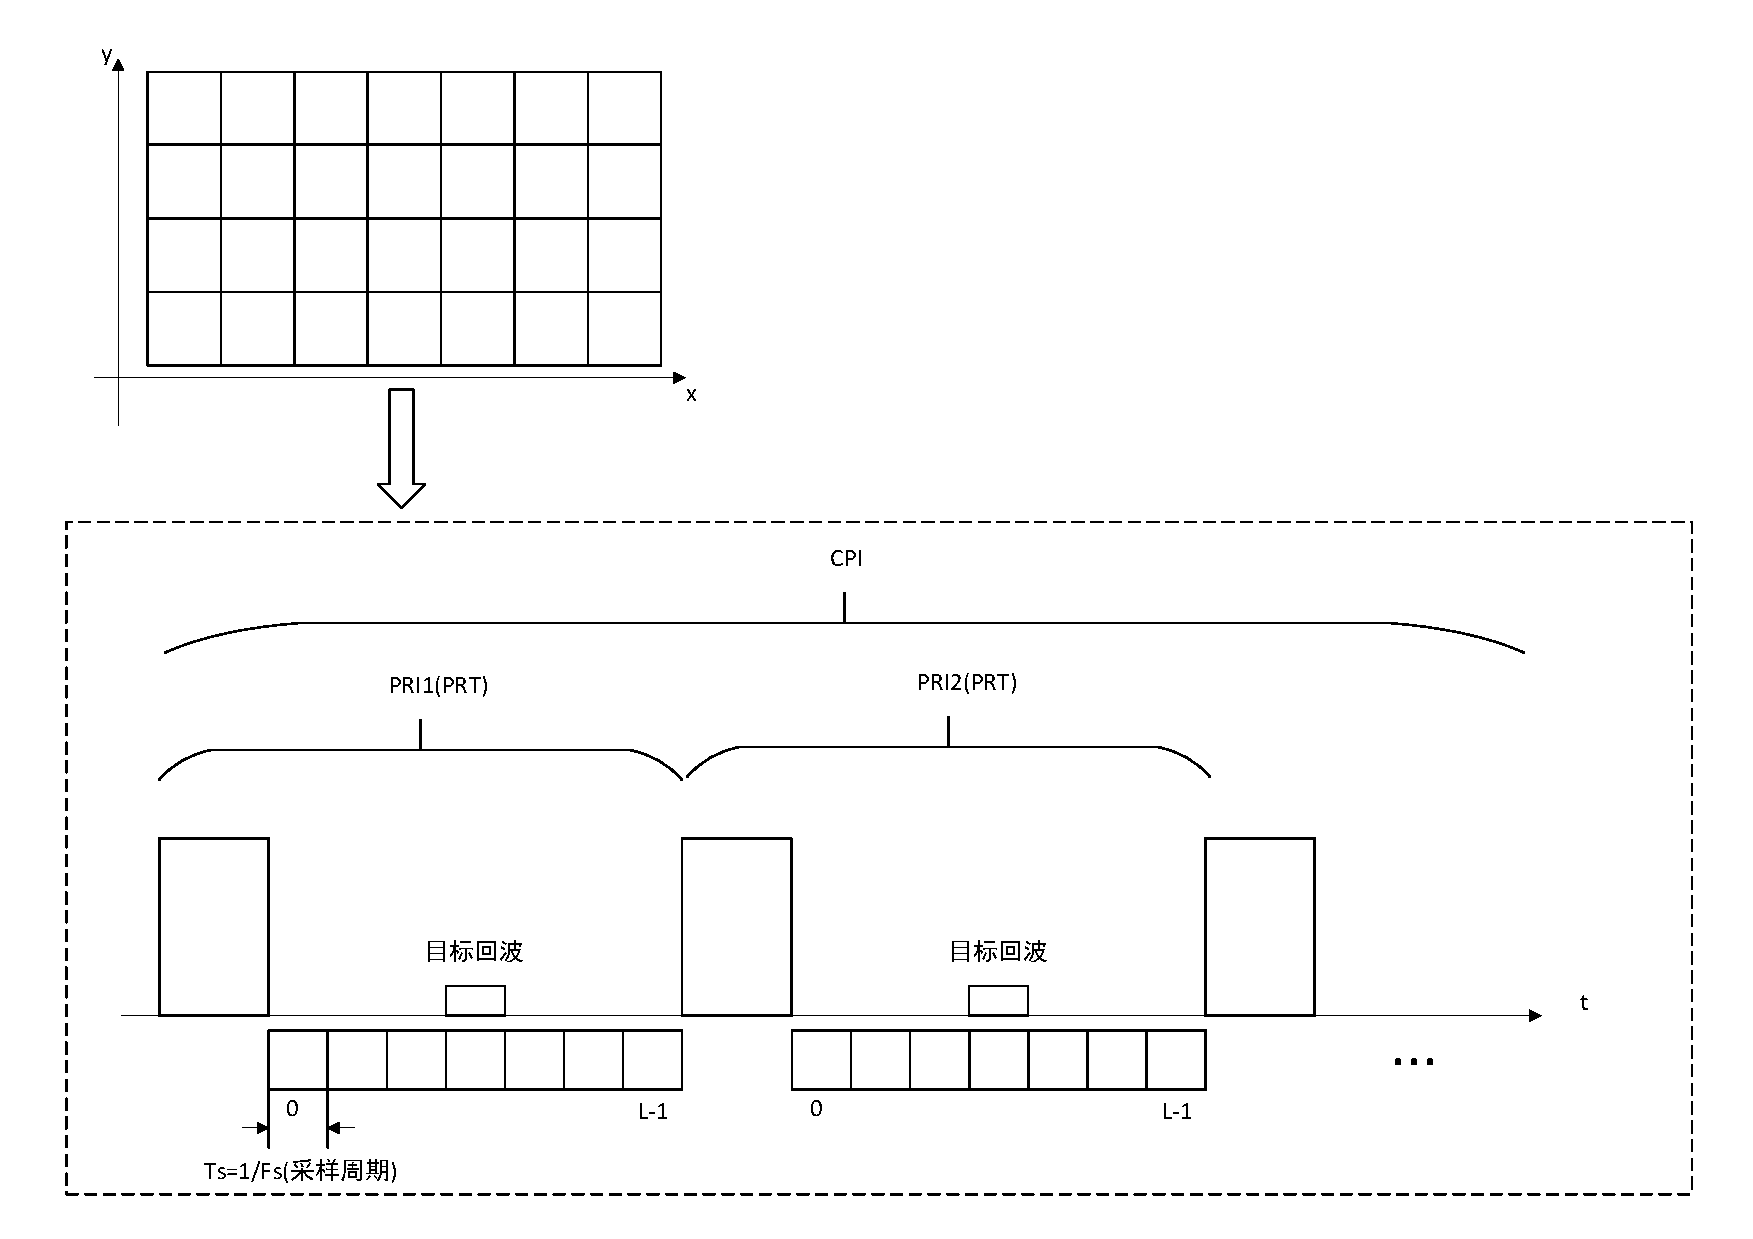
\includegraphics [width=1.0\textwidth]{figure//CPIdata.pdf}
    \caption{CPI数据}\label{CPIdata}
\end{figure}

根据上面两节的叙述基本建立了一个数据处理的模型,后面的计算和处理均会在这个三维模型来进行
展开。

\section{指标算法}
有了数据处理模型,还需要知道如何处理这个数据模型,现在就像做菜,菜的原材料已经有了,但是
还需要食谱,然后根据食谱做出想吃的菜,本节就是描述如何进行处理这些原材料。首先需要面对的
就是3个最基本的指标,反射率强度(Z),径向速度(V),速度谱宽(W),下面就逐个指标来进行计算。

\subsection{反射率强度}
反射率强度(Z)是雷达回波的最基本指标,在这里主要引用
《雷达信号处理基础(第二版)》\cite{FundamentalsOfRadarSignalProcessing}中2.2.4节中的
计算模型,雷达气象学通常采用称为反射率的归一化因子来表示气象目标的散射特性,通常用Z表示,
体反射率(RCS)公式如下:

\begin{proposition}[体反射率]

    \begin{equation}
        \eta=\frac{\pi^5|K|^2}{\lambda}Z
    \end{equation}

    $|K^2|$:对于由水构成的散射体其值近似为0.93,由冰构成的散射体近似为0.197

    $\lambda$:雷达波长

\end{proposition}

当给出一个回波功率测量值,就可以用雷达方程估计出$\eta$,然后利用公式2.1换算成Z,再
对取10lgZ即得到dBZ。

《雷达信号处理基础(第二版)》\cite{FundamentalsOfRadarSignalProcessing}中2.2.2节给出
的体散射目标的雷达方程如下:
\begin{proposition}[体散射雷达方程]

    \begin{equation}
        p_r\left(t_0\right)=\frac{P_tG^2\lambda^2\eta\Delta R\theta_3\phi_3}{
                            \left(4\pi\right)^3R_0^2L_sL_a\left(R_0\right)}
    \end{equation}

    $p_r(t_0)$:$t_0$时刻回波接收功率

    $P_t$:雷达辐射功率

    $G$:天线增益

    $\lambda$:雷达波长

    $\Delta R$:一个距离分辨单元的长度

    $\theta_3$:方位3dB波束宽度

    $\phi_3$:俯仰3dB波束宽度

    $R_0$:分辨单元中心距离

    $L_s$:系统损耗因子

    $L_a(R_0)$:$R_0$处的大气衰减
\end{proposition}

根据公式2.1和2.2便可以解出Z,综合后的公式如下:
\begin{proposition}[体散射雷达方程]

    \begin{equation}
        Z=\frac{64}{\pi^2}*\frac{L_sL_a\left(R_0\right)}
            {P_tG^2\lambda|K|^2\Delta R\theta_3\phi_3}*R_0^2P_r(t_0)
    \end{equation}

\end{proposition}

根据公式2.3可以看出只要从上一节中的距离库获取$R_0$和$P_r(t_0)$便可以解出Z的值,公式中
的其它部分则可以根据相关的系统属性计算为一个常数。

$R_0$的值是比较好计算的,直接使用下面的公式:
\begin{proposition}[目标距离计算]

    \begin{equation}
        R_0=\frac{c*t_0}{2} 
    \end{equation}

    $c$:光速

    $t_0$:接收机接收回波的时间

\end{proposition}

下面重点介绍一下$P_r(t_0)$的计算,为了得到更好的信噪比,回波功率需要在一个CPI上来计算信
号功率,相干积累可以增加信噪比主要源于下面三个公式。

\begin{proposition}[相干积累]

    \begin{equation}
        \chi_1=\frac{A^2}{\sigma_w^2}
    \end{equation}

    \begin{equation}
        \sum_{n=0}^{N-1}\left\{Ae^{j\phi}+w\left[n\right]\right\}=NAe^{j\phi}+\sum_{n=0}^{N-1}w\left[n\right]
    \end{equation}

    \begin{equation}
        \chi_N=\frac{(NA)^2}{N\sigma_w^2}=N\chi_1
    \end{equation}

    $\chi_1$:单脉冲的SNR

    $A$:复回波$Ae^{j\phi}$的幅度值

    $\Sigma_w^2$:随机噪声的信号功率

    $w[n]$:噪声信号

    $\chi_N$:N个相干信号累计的SNR

\end{proposition}


\subsection{径向速度}

\subsection{速度谱宽}


%\begin{figure}[hbtp]
%    \centering
%    \includegraphics [width=0.8\textwidth]{figure//NetSoft.pdf}
%    \caption{C/S架构图}\label{NetSoft}
%\end{figure}

在基本的框架符合经典C/S架构的情况下,本文将采用大量现有的成熟框架进行服务端和设备客户端
的设计,在设备端将会采用curl工具开发,服务端则采用开源框架根据需求定制开发,客户端则通过
浏览器登录远程服务器界面进行人机交互。

\end{spacing}

%---------------------------------------------------------------------
%  第三章 模块设计
%---------------------------------------------------------------------
\chapter{设计实现}
\begin{spacing}{1.5}
\songti\zihao{-4}

\section{服务器端}
\subsection{功能设计}
服务器端的基本功能主要有三个:

\begin{itemize}
    \itemsep=3pt
    \parskip=0pt
    \setlength{\itemindent}{1em}
    \item 处理设备端消息
    \item 处理客户端消息
    \item 数据存储管理
\end{itemize}

如图3.1所示,更加形象的描述了服务端的业务逻辑功能。
%\begin{figure}[hbtp]
%    \centering
%    \includegraphics [width=0.8\textwidth]{figure//NetServer.pdf}
%    \caption{服务器功能设计}\label{NetServer}
%\end{figure}

在我们的使用场景中设备端和客户端一般都是是处于内网,服务端则分配有公网IP地址,因此设备端
和客户端均会主动向服务端发起连接,设备端主要将自身的数据信息发送给服务端,服务端接收数据
之后将数据存储到数据库,等待客户端的查询。在本文中拟采用的rttys同时提供了客户端直接获取
设备端数据的接口,可以即时操作即时获取相关设备端数据。


\subsection{接口设计}
本节主要对服务端与设备端和客户端的通信接口进行详细设计。
\begin{enumerate}[(1)]
    \itemsep=3pt
    \parskip=0pt
    \setlength{\itemindent}{2em}
    \item 设备端接口

        设备端接口设计成符合HTTP规范的标准接口,接口如下所示:
        \begin{tcolorbox}[notitle,boxrule=0pt,colback=blue!20,colframe=blue!20]
            https://Server-ip:port/devs
        \end{tcolorbox}

        设备端通过服务器提供的devs接口采用标准post的方式将自己所收集的数据传输给远端服
        务器,服务器收到数据之后再将其存储起来。
    \item 客户端接口

        客户端接口同样也是设计成符合HTTP规范的标准接口,接口如下所示:
        \begin{tcolorbox}[notitle,boxrule=0pt,colback=blue!20,colframe=blue!20]
            https://Server-ip:port/clients
        \end{tcolorbox}
        服务器端clients接口提供给客户端访问的接口,客户端通过clients访问指定的设备,获
        取设备信息。
    \item 即时通讯接口
        客户端通过即时通讯接口可以直接的访问设备端的内容,连接设备的shell命令行,执行相
        关的设备端命令。
        \begin{tcolorbox}[notitle,boxrule=0pt,colback=blue!20,colframe=blue!20]
            https://Server-ip:port/cmd \cite{rtty.web}
        \end{tcolorbox}

\end{enumerate}


\section{设备端}
\subsection{功能设计}
设备端的功能则相对比较简单,主要是通过curl工具根据通信协议将网关设备的信息和与网关设备相
连接的设备的消息传递给给服务器端,同时从服务器端下载设备配置文件。

%\begin{figure}[H]
%    \centering
%    \includegraphics [width=1.0\textwidth]{figure//DevLogic.pdf}
%    \caption{设备端基本功能}\label{DevLogic}
%\end{figure}

设备端基本功能和程序处理逻辑如图3.2所示,通过定时维护与服务器的数据传递,获取配置文件和
将收集的网关、UPS和摄像头等设备的数据传输给服务器端,同时比较从服务器端下载的配置文件与
当前配置文件,如果配置文件有变化,则解析配置文件配置设备对应的项目。

\subsection{接口设计}
设备端接口设计成符合HTTP规范的标准接口,接口如下所示:
    \begin{tcolorbox}[notitle,boxrule=0pt,colback=blue!20,colframe=blue!20]
        \quad https://Server-ip:port/devs
    \end{tcolorbox}

设备端通过服务器提供的devs接口采用标准post的方式将自己所收集的数据传输给远端服务器,服
务器收到数据之后再将其存储起来,同时post的过程中获取服务器的设备配置文件,并和本地文件相
比较,如果没有变化的不进行设备配置,如果配置文件有变化的配置相应的项目。

\section{客户端}
\subsection{功能设计}
在本文中客户端的设计主要采取使用者直接通过浏览器软件登录远程服务器Web进行进行人际交互的
方式进行,但是考虑到后期可能会有需要将设备管理嵌入到PC端软件或者手机端APP的需求,设计时
预留客户端接口,通过客户端接口,可以获取对应的设备节点的信息,并且通过该接口也可以设置对
应的网关设备。基本功能如图3.3所示。
%\begin{figure}[H]
%    \centering
%    \includegraphics [width=0.8\textwidth]{figure//Netclient.pdf}
%    \caption{客户端基本功能}\label{Netclient}
%\end{figure}

\subsection{接口设计}
客户端接口同样也是设计成符合HTTP规范的标准接口,接口如下所示:
\begin{tcolorbox}[notitle,boxrule=0pt,colback=blue!20,colframe=blue!20]
    \quad https://Server-ip:port/clients
\end{tcolorbox}
服务器端clients接口提供给客户端访问的接口,客户端通过clients访问指定的设备,获
取设备信息。
\end{spacing}

%---------------------------------------------------------------------
%  第四章 协议设计
%---------------------------------------------------------------------
\chapter{详细设计}
\begin{spacing}{1.5}       

本章的协议设计是针对上一章所设计的通讯接口的补充,更加详细描述了通讯接口传输的数据内容和格
式。
\begin{enumerate}[(1)]
    \itemsep=3pt
    \parskip=0pt
    \setlength{\itemindent}{2em}
    \item 设备端通讯协议
       
        设备端与服务器通信的协议格式如下:
        \begin{tcolorbox}[notitle,boxrule=0pt,colback=gray!20,colframe=blue!20]
            \{

                "DevId"  : id-number,

                "Status" : status-id,

                "name"   : "Dev name",

                "Discrip": "Dev discription",

                "locate" : "position",
                
                "time"   : "time",

                "date"   : "xxxx-xx-xx",

                "data"   : [

                    \quad\{

                        \quad\quad"name"   : "son dev name",

                        \quad\quad"status" : status-id,

                        \quad\quad"discrip": "Dev discription",

                        \quad\quad"data"   : [],

                    \quad\},

                    \quad...
                    
                ]

            \}
        \end{tcolorbox}
        通信协议格式采用标准的json格式,协议内部需要包含设备状态信息和挂载的子设备状态
        信息。
        
    \item 客户端接口

        客户端接口则是通过client获取从服务器获取设备相关的数据和信息,接口协议如下所示:
        \begin{tcolorbox}[notitle,boxrule=0pt,colback=gray!20,colframe=blue!20]
            \{

                "target-id"  : id-number,

                "Status" : status-id,

                "name"   : "Dev name",

                "Discrip": "Dev discription",

                "locate" : "position",
                
                "time"   : "time",

                "date"   : "xxxx-xx-xx",

                "data"   : [

                    \quad\{

                        \quad\quad"name"   : "son dev name",

                        \quad\quad"status" : status-id,

                        \quad\quad"discrip": "Dev discription",

                        \quad\quad"data"   : [],

                    \quad\},

                    \quad...
                    
                ]

            \}
        \end{tcolorbox}

    \item 即时通讯协议

        客户端通过即时通讯接口协议是rtty框架提供的一个直接访问设备的方式,这里参考rtty
        框架提供的协议,如下所示:
        \begin{tcolorbox}[notitle,boxrule=0pt,colback=gray!20,colframe=blue!20]
            curl -k https://server-ip:5912/cmd -d '\{"devid":"test","username":"test",

            "password":"123456","cmd":"ls","params":["/"],"env":\{\}\}'
        \end{tcolorbox}

\end{enumerate}

\end{spacing}
%---------------------------------------------------------------------
%  第四章 总结
%---------------------------------------------------------------------
\chapter{总结}
\begin{spacing}{1.5}       
    整个网关网络管理还是比较纷繁复杂的,主要是因为设备分散,且网关后面又连接了一定数量的
    子设备,且网关一般是位于内网,需要穿透公网对网络设备进行网络管理和配置,本文基于功能
    需求的考虑,结合将要使用的实际环境,参考了rtty和rttys\cite{rtty.web}等开源反向代理程序框架进行方案
    设计。
\end{spacing}

%---------------------------------------------------------------------
%  参考文献设置
%---------------------------------------------------------------------
\addcontentsline{toc}{chapter}{参考文献}

\begin{thebibliography}{99}
\songti \zihao{-4} 	
    \bibitem{rtty.web}
    https://github.com/zhaojh329/rtty
    \bibitem{rttys.web}
    https://github.com/zhaojh329/rttys
    \bibitem{snmp.web}
    https://tools.ietf.org/html/rfc5343
    \bibitem{FundamentalsOfRadarSignalProcessing}
    Mark A.Richards . 雷达信号处理基础 (第二版) [M]. 2008.
    
	
\end{thebibliography}

\end{document}